\documentclass{ximera}

%\usepackage{todonotes}

\newcommand{\todo}{}

\usepackage{tkz-euclide}
\tikzset{>=stealth} %% cool arrow head
\tikzset{shorten <>/.style={ shorten >=#1, shorten <=#1 } } %% allows shorter vectors

\usepackage{tkz-tab}  %% sign charts
\usetikzlibrary{decorations.pathreplacing} 

\usetikzlibrary{backgrounds} %% for boxes around graphs
\usetikzlibrary{shapes,positioning}  %% Clouds and stars
\usetikzlibrary{matrix} %% for matrix
\usepgfplotslibrary{polar} %% for polar plots
\usetkzobj{all}
\usepackage[makeroom]{cancel} %% for strike outs
%\usepackage{mathtools} %% for pretty underbrace % Breaks Ximera
\usepackage{multicol}

\usepackage{polynom}



\usepackage[many]{tcolorbox}  %% for titled boxes
\newtcolorbox{xbox}[1]{%
    tikznode boxed title,
    enhanced,
    arc=0mm,
    interior style={white},
    attach boxed title to top center= {yshift=-\tcboxedtitleheight/2},
    fonttitle=\bfseries,
    colbacktitle=white,coltitle=black,
    boxed title style={size=normal,colframe=white,boxrule=0pt},
    title={#1}}


\usepackage{array}
\setlength{\extrarowheight}{+.1cm}   
\newdimen\digitwidth
\settowidth\digitwidth{9}
\def\divrule#1#2{
\noalign{\moveright#1\digitwidth
\vbox{\hrule width#2\digitwidth}}}





\newcommand{\RR}{\mathbb R}
\newcommand{\R}{\mathbb R}
\newcommand{\N}{\mathbb N}
\newcommand{\Z}{\mathbb Z}

%\renewcommand{\d}{\,d\!}
\renewcommand{\d}{\mathop{}\!d}
\newcommand{\dd}[2][]{\frac{\d #1}{\d #2}}
\newcommand{\pp}[2][]{\frac{\partial #1}{\partial #2}}
\renewcommand{\l}{\ell}
\newcommand{\ddx}{\frac{d}{\d x}}
\newcommand{\ddt}{\frac{d}{\d t}}

\newcommand{\zeroOverZero}{\ensuremath{\boldsymbol{\tfrac{0}{0}}}}
\newcommand{\inftyOverInfty}{\ensuremath{\boldsymbol{\tfrac{\infty}{\infty}}}}
\newcommand{\zeroOverInfty}{\ensuremath{\boldsymbol{\tfrac{0}{\infty}}}}
\newcommand{\zeroTimesInfty}{\ensuremath{\small\boldsymbol{0\cdot \infty}}}
\newcommand{\inftyMinusInfty}{\ensuremath{\small\boldsymbol{\infty - \infty}}}
\newcommand{\oneToInfty}{\ensuremath{\boldsymbol{1^\infty}}}
\newcommand{\zeroToZero}{\ensuremath{\boldsymbol{0^0}}}
\newcommand{\inftyToZero}{\ensuremath{\boldsymbol{\infty^0}}}



\newcommand{\numOverZero}{\ensuremath{\boldsymbol{\tfrac{\#}{0}}}}
\newcommand{\dfn}{\textbf}
%\newcommand{\unit}{\,\mathrm}
\newcommand{\unit}{\mathop{}\!\mathrm}
\newcommand{\eval}[1]{\bigg[ #1 \bigg]}
\newcommand{\seq}[1]{\left( #1 \right)}
\renewcommand{\epsilon}{\varepsilon}
\renewcommand{\iff}{\Leftrightarrow}

\DeclareMathOperator{\arccot}{arccot}
\DeclareMathOperator{\arcsec}{arcsec}
\DeclareMathOperator{\arccsc}{arccsc}
\DeclareMathOperator{\si}{Si}
\DeclareMathOperator{\proj}{proj}
\DeclareMathOperator{\scal}{scal}


\newcommand{\tightoverset}[2]{% for arrow vec
  \mathop{#2}\limits^{\vbox to -.5ex{\kern-0.75ex\hbox{$#1$}\vss}}}
\newcommand{\arrowvec}[1]{\tightoverset{\scriptstyle\rightharpoonup}{#1}}
\renewcommand{\vec}{\mathbf}
\newcommand{\veci}{\vec{i}}
\newcommand{\vecj}{\vec{j}}
\newcommand{\veck}{\vec{k}}
\newcommand{\vecl}{\boldsymbol{\l}}

\newcommand{\dotp}{\bullet}
\newcommand{\cross}{\boldsymbol\times}
\newcommand{\grad}{\boldsymbol\nabla}
\newcommand{\divergence}{\grad\dotp}
\newcommand{\curl}{\grad\cross}
%\DeclareMathOperator{\divergence}{divergence}
%\DeclareMathOperator{\curl}[1]{\grad\cross #1}


\colorlet{textColor}{black} 
\colorlet{background}{white}
\colorlet{penColor}{blue!50!black} % Color of a curve in a plot
\colorlet{penColor2}{red!50!black}% Color of a curve in a plot
\colorlet{penColor3}{red!50!blue} % Color of a curve in a plot
\colorlet{penColor4}{green!50!black} % Color of a curve in a plot
\colorlet{penColor5}{orange!80!black} % Color of a curve in a plot
\colorlet{fill1}{penColor!20} % Color of fill in a plot
\colorlet{fill2}{penColor2!20} % Color of fill in a plot
\colorlet{fillp}{fill1} % Color of positive area
\colorlet{filln}{penColor2!20} % Color of negative area
\colorlet{fill3}{penColor3!20} % Fill
\colorlet{fill4}{penColor4!20} % Fill
\colorlet{fill5}{penColor5!20} % Fill
\colorlet{gridColor}{gray!50} % Color of grid in a plot

\newcommand{\surfaceColor}{violet}
\newcommand{\surfaceColorTwo}{redyellow}
\newcommand{\sliceColor}{greenyellow}




\pgfmathdeclarefunction{gauss}{2}{% gives gaussian
  \pgfmathparse{1/(#2*sqrt(2*pi))*exp(-((x-#1)^2)/(2*#2^2))}%
}


%%%%%%%%%%%%%
%% Vectors
%%%%%%%%%%%%%

%% Simple horiz vectors
\renewcommand{\vector}[1]{\left\langle #1\right\rangle}


%% %% Complex Horiz Vectors with angle brackets
%% \makeatletter
%% \renewcommand{\vector}[2][ , ]{\left\langle%
%%   \def\nextitem{\def\nextitem{#1}}%
%%   \@for \el:=#2\do{\nextitem\el}\right\rangle%
%% }
%% \makeatother

%% %% Vertical Vectors
%% \def\vector#1{\begin{bmatrix}\vecListA#1,,\end{bmatrix}}
%% \def\vecListA#1,{\if,#1,\else #1\cr \expandafter \vecListA \fi}

%%%%%%%%%%%%%
%% End of vectors
%%%%%%%%%%%%%

%\newcommand{\fullwidth}{}
%\newcommand{\normalwidth}{}



%% makes a snazzy t-chart for evaluating functions
%\newenvironment{tchart}{\rowcolors{2}{}{background!90!textColor}\array}{\endarray}

%%This is to help with formatting on future title pages.
\newenvironment{sectionOutcomes}{}{} 



%% Flowchart stuff
%\tikzstyle{startstop} = [rectangle, rounded corners, minimum width=3cm, minimum height=1cm,text centered, draw=black]
%\tikzstyle{question} = [rectangle, minimum width=3cm, minimum height=1cm, text centered, draw=black]
%\tikzstyle{decision} = [trapezium, trapezium left angle=70, trapezium right angle=110, minimum width=3cm, minimum height=1cm, text centered, draw=black]
%\tikzstyle{question} = [rectangle, rounded corners, minimum width=3cm, minimum height=1cm,text centered, draw=black]
%\tikzstyle{process} = [rectangle, minimum width=3cm, minimum height=1cm, text centered, draw=black]
%\tikzstyle{decision} = [trapezium, trapezium left angle=70, trapezium right angle=110, minimum width=3cm, minimum height=1cm, text centered, draw=black]


\outcome{Define continuity in terms of limits.}
\outcome{Calculate limits using the limit laws.}
\outcome{Famous functions are continuous on their domains.}

\title[Dig-In:]{Continuity}
\begin{document}
\begin{abstract}
Continuity is defined by limits. 
\end{abstract}
\maketitle


Limits are simple to compute when they can be found by plugging the
value into the function.  That is, when
\[
\lim_{x\to c}f(x) = f(c).
\]
We call this property \textit{continuity}.

\begin{definition}
  A function $f$ is \dfn{continuous at a point} $a$ if
  \[
  \lim_{x\to a}f(x) = f(a).
  \]
\end{definition}

\begin{question}
  Consider the graph of $y=f(x)$ below
  \begin{image}
    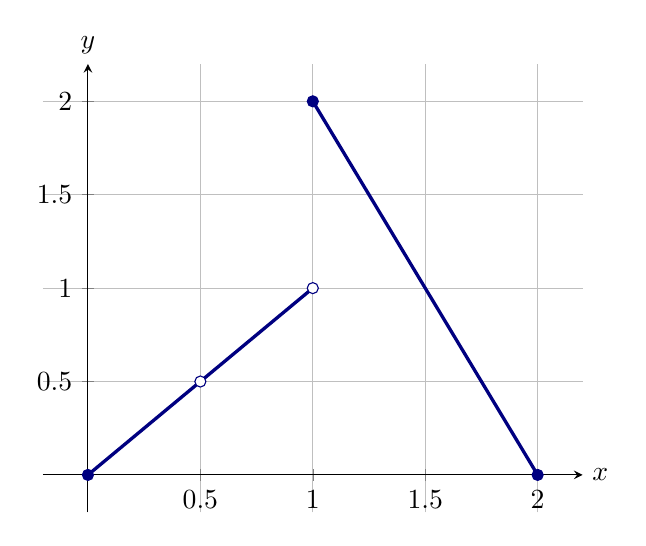
\begin{tikzpicture}
      \begin{axis}
	[xmin=-0.2,
          xmax=2.2,
          ymin=-0.2,
          ymax=2.2,
          axis lines=center,
          xlabel=$x$,ylabel=$y$,
          every axis y label/.style={at=(current axis.above origin),anchor=south},
          every axis x label/.style={at=(current axis.right of origin),anchor=west},
	  domain=-1:2,
          clip=false,
	  ytick={0.5,1,1.5,2},
	  yticklabels={$0.5$,$1$,$1.5$,$2$},
	  xtick={0.5,1.0,1.5,2},
	  xticklabels={$0.5$,$1$,$1.5$,$2$},
	  grid = major
	]
        \addplot[very thick,penColor] plot coordinates {(0,0) (1,1)};
        \addplot[very thick,penColor] plot coordinates {(1,2) (2,0)};
        
        %\draw[very thin,color=black] (axis cs:0,-0.2) -- (axis cs:0,2);

        \addplot[color=penColor,fill=background,only marks,mark=*] coordinates{(1,1)};  %% open hole
        \addplot[color=penColor,fill=background,only marks,mark=*] coordinates{(.5,.5)};  %% open hole

        \addplot[color=penColor,fill=penColor,only marks,mark=*] coordinates{(0,0)};  %% closed hole
        \addplot[color=penColor,fill=penColor,only marks,mark=*] coordinates{(2,0)};  %% closed hole
        \addplot[color=penColor,fill=penColor,only marks,mark=*] coordinates{(1,2)};  %% closed hole
        
        %% \draw[fill=black] (axis cs:0,0) circle [radius=2pt];
	%% \draw[fill=black] (axis cs:2,0) circle [radius=2pt];
        %% \draw[fill=black] (axis cs:1,2) circle [radius=2pt];
	
	\end{axis}
    \end{tikzpicture}
  \end{image}
  Which of the following are true?
  \begin{multipleChoice}
    \choice{$f$ is continuous at $x=0.5$}
    \choice{$f$ is continuous at $x=1$}
    \choice[correct]{$f$ is continuous at $x=1.5$}
  \end{multipleChoice}
  
\end{question}

It is very important to note that saying
\begin{center}
  ``a function $f$ is continuous at a point $a$''
\end{center}
is really making \textbf{three} statements:
%\begin{xbox}{$f$ is continuous at $a$ means:}
	\begin{enumerate}
		\item $f(a)$ is defined.  That is, $a$ is in the domain of $f$.
		\item $\lim_{x\to a} f(x)$ exists.
		\item $\lim_{x\to a} f(x) = f(a)$.
	\end{enumerate}
%\end{xbox}

The first two of these statements are implied by the third statement, but are important enough that we want to 
break them up to highlight their significance.

\begin{example}
Find the discontinuities (the points $x$ where a function is not
continuous) for the function described below:
\begin{image}
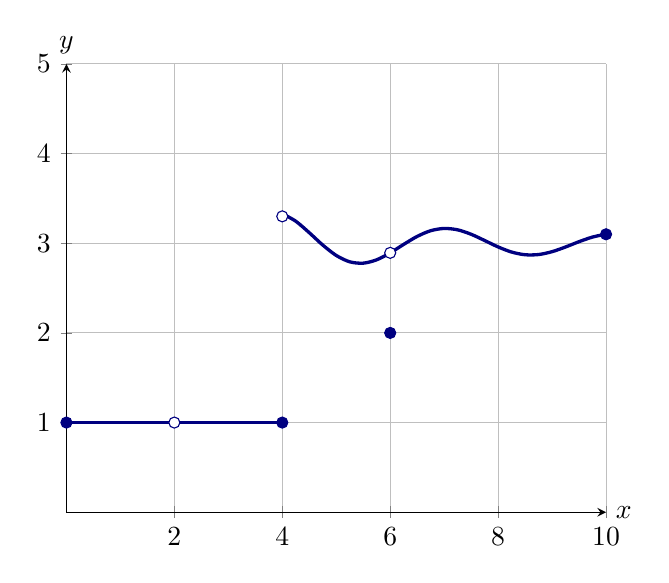
\begin{tikzpicture}
	\begin{axis}[
            domain=0:10,
            ymax=5,
            ymin=0,
            %samples=100,
            axis lines =middle, xlabel=$x$, ylabel=$y$,
            every axis y label/.style={at=(current axis.above origin),anchor=south},
            every axis x label/.style={at=(current axis.right of origin),anchor=west},
            %% ytick={0.5,1,1.5,2},
	    %% yticklabels={$0.5$,$1$,$1.5$,$2$},
	    %% xtick={0.5,1.0,1.5,2},
	    %% xticklabels={$0.5$,$1$,$1.5$,$2$},
	    grid = major
          ]
	  \addplot [very thick, penColor, smooth, domain=(4:10)] {3 + sin(deg(x*2))/(x-1)};
          \addplot [very thick, penColor, smooth, domain=(0:4)] {1};
          \addplot[color=penColor,fill=background,only marks,mark=*] coordinates{(4,3.30)};  %% open hole
          \addplot[color=penColor,fill=background,only marks,mark=*] coordinates{(2,1)};  %% open hole
          \addplot[color=penColor,fill=background,only marks,mark=*] coordinates{(6,2.893)};  %% open hole
          \addplot[color=penColor,fill=penColor,only marks,mark=*] coordinates{(4,1)};  %% closed hole
          \addplot[color=penColor,fill=penColor,only marks,mark=*] coordinates{(6,2)};  %% closed hole

          \addplot[color=penColor,fill=penColor,only marks,mark=*] coordinates{(0,1)};  %% closed hole
          \addplot[color=penColor,fill=penColor,only marks,mark=*] coordinates{(10,3.1)};  %% closed hole
        \end{axis}
\end{tikzpicture}
%% \caption{A plot of a function with discontinuities at $x=4$ and $x=6$.}
%% \label{plot:discontinuous-function}
\end{image}

\begin{explanation}
  To start, $f$ is not even defined at $x=\answer[given]{2}$, hence $f$
  cannot be continuous at $x=\answer[given]{2}$.

  Next, from the plot above we see that $\lim_{x\to 4} f(x)$ does not
  exist because
  \[
  \lim_{x\to 4^-}f(x) = \answer[given]{1}\qquad\text{and}\qquad \lim_{x\to 4^+}f(x) \approx \answer[given,tolerance=1]{3.5}
  \]
  Since $\lim_{x\to 4} f(x)$ does not exist, $f$ cannot be continuous
  at $x=4$.

  We also see that $\lim_{x\to 6} f(x) \approx
  \answer[given,tolerance=.5]{3}$ while $f(6) =
  \answer[given]{2}$. Hence $\lim_{x\to 6} f(x) \ne f(6)$, and so $f$
  is not continuous at $x=6$.
\end{explanation}
\end{example}


Building from the definition of \textit{continuity at a point}, we can
now define what it means for a function to be \textit{continuous} on
an open interval.

\begin{definition}
  A function $f$ is \dfn{continuous on an open interval} $I$ if
  $\lim_{x\to a} f(x) = f(a)$ for all $a$ in $I$.
\end{definition}

Loosely speaking, a function is continuous on an interval $I$ if you
can draw the function on that interval without any breaks in the
graph.  This is often referred to as being able to draw the graph
``without picking up your pencil.''

\begin{theorem}[Continuity of Famous Functions]\index{continuity of famous functions}\label{theorem:continuity}
The following functions are continuous on the given intervals for $k$ a real number and $b$ a positive real number:
\begin{description}
	\item[Constant function]\index{constant function} $f(x) =k$ is continuous on $(-\infty , \infty )$.
	\item[Identity function]\index{indenity function} $f(x) = x$ is continuous on $(-\infty , \infty)$.
	\item[Power function]\index{power function} $f(x)=x^b$ is continuous on $(-\infty , \infty)$.
	\item[Exponential function]\index{exponential function} $f(x)=b^x$ is continuous on $(-\infty , \infty)$.
	\item[Logarithmic function]\index{logarithmic function} $f(x)=\log_b(x)$ is continuous on $(0 , \infty)$.
	\item[Sine and cosine] Both $\sin(x)$ and $\cos(x)$ are continuous on $(-\infty , \infty)$.\index{sine}\index{cosine}
\end{description}
In essence, we are saying that the functions listed above are
continuous wherever they are defined, that is, on their natural
domains.
\end{theorem}


\begin{question}
  Compute:
  $\lim_{x\to 3} x^\pi \begin{prompt}= \answer{3^\pi}\end{prompt}$
  \begin{feedback}
    The function $f(x)=x^\pi$ is of the form $x^k$ for a real number
    $k$.  Therefore, $f(x)=x^\pi$ is continuous for all real values of
    $x$.  In particular, $f(x)$ is continuous at $x=3$.  Since $x^\pi$
    is continuous at $3$, we know that $\lim_{x\to 3} f(x) = f(3)$.
    That is, $\lim_{x\to 3} x^\pi = 3^\pi$
  \end{feedback}  
\end{question}

\section{Left and right continuity}


At this point we have a small problem.  For functions such as
$\sqrt{x}$, the natural domain is $0\leq x <\infty$.  This is not an
open interval.  What does it mean to say that $\sqrt{x}$ is continuous
at $0$ when $\sqrt{x}$ is not defined for $x<0$? To get us out of this
quagmire, we need a new definition:

\begin{definition}
  A function $f$ is \dfn{left continuous} at a point $a$ if
  $\lim_{x\to a^-} f(x) = f(a)$.

  A function $f$ is \dfn{right continuous} at a point $a$ if
  $\lim_{x\to a^+} f(x) = f(a)$.
\end{definition}

Now we can say that a function is continuous at a left endpoint of an
interval if it is right continuous there, and a function is continuous
at the right endpoint of an interval if it is left continuous
there. This allows us to talk about continuity on closed intervals.


\begin{definition}
  A function $f$ is
  \begin{itemize}
    \item \dfn{continuous on a closed interval} $[a,b]$ if $f$ is
      continuous on $(a,b)$, right continuous at $a$, and left
      continuous at $b$;
    \item \dfn{continuous on a half-closed interval} $[a,b)$ if $f$ is
      continuous on $(a,b)$ and right continuous at $a$;
    \item \dfn{continuous on a half-closed interval} $(a,b]$ if $f$ is
      $f$ is continuous on $(a,b)$ and left continuous at $b$.
  \end{itemize}
\end{definition}



\begin{question}
Here we give the graph of a function defined on $[0,10]$.
\begin{image}
\begin{tikzpicture}
	\begin{axis}[
            domain=0:10,
            ymax=5,
            ymin=0,
            samples=100,
            axis lines =middle, xlabel=$x$, ylabel=$y$,
            every axis y label/.style={at=(current axis.above origin),anchor=south},
            every axis x label/.style={at=(current axis.right of origin),anchor=west}
          ]
	  \addplot [very thick, penColor, smooth, domain=(4:10)] {3 + sin(deg(x*2))/(x-1)};
          \addplot [very thick, penColor, smooth, domain=(0:4)] {1};
          \addplot[color=penColor,fill=background,only marks,mark=*] coordinates{(4,3.30)};  %% open hole
          \addplot[color=penColor,fill=background,only marks,mark=*] coordinates{(6,2.893)};  %% open hole
          \addplot[color=penColor,fill=penColor,only marks,mark=*] coordinates{(4,1)};  %% closed hole
          \addplot[color=penColor,fill=penColor,only marks,mark=*] coordinates{(6,2)};  %% closed hole
          \addplot[color=penColor,fill=penColor,only marks,mark=*] coordinates{(0,1)};  %% closed hole
          \addplot[color=penColor,fill=penColor,only marks,mark=*] coordinates{(10,3.1)};  %% closed hole
        \end{axis}
\end{tikzpicture}
%% \caption{A plot of a function with discontinuities at $x=4$ and $x=6$.}
%% \label{plot:discontinuous-function}
\end{image}
What are the largest intervals of continuity for this function?
\begin{multipleChoice}
  \choice{$[0,10]$}
  \choice{$[0,4)$ and $(4,10]$}
  \choice{$[0,4]$, $[4,6]$, and $[6,10]$}
  \choice{$(0,4)$, $(4,6)$, and $(6,10)$}
  \choice{$[0,4]$, $(4,6)$, and $[6,10]$}
  \choice[correct]{$[0,4]$, $(4,6)$, and $(6,10]$}
  \choice{$[0,4)$, $(4,6)$, and $(6,10]$}
  \choice{$(0,4]$, $[4,6]$, and $[6,10)$}
\end{multipleChoice}
\begin{feedback}
Notice that our function is left continuous at $x=4$ so we can include
$4$ in the interval $[0,4]$. Four is not included in the interval
$(4,6)$ because our function is not right continuous at $x=4$.
Similarly, our function is neither right or left continuous at $x=6$,
so $6$ is not included in any intervals.  Our function is left
continuous at $x=0$ and right continuous at $x=10$ so we included
these endpoints in our intervals.
\end{feedback}
\end{question}



\end{document}

